\documentclass[tikz]{standalone}
\usepackage[utf8]{inputenc}
\usepackage{xcolor}

\usetikzlibrary{positioning}
\usetikzlibrary{shapes.geometric}
\usetikzlibrary {arrows.meta}
\usetikzlibrary {fit}

\definecolor{cyellow}{HTML}{E0BA4F}
\definecolor{cpurple}{HTML}{7E74AC}
\definecolor{corange}{HTML}{D17638}

\begin{document}
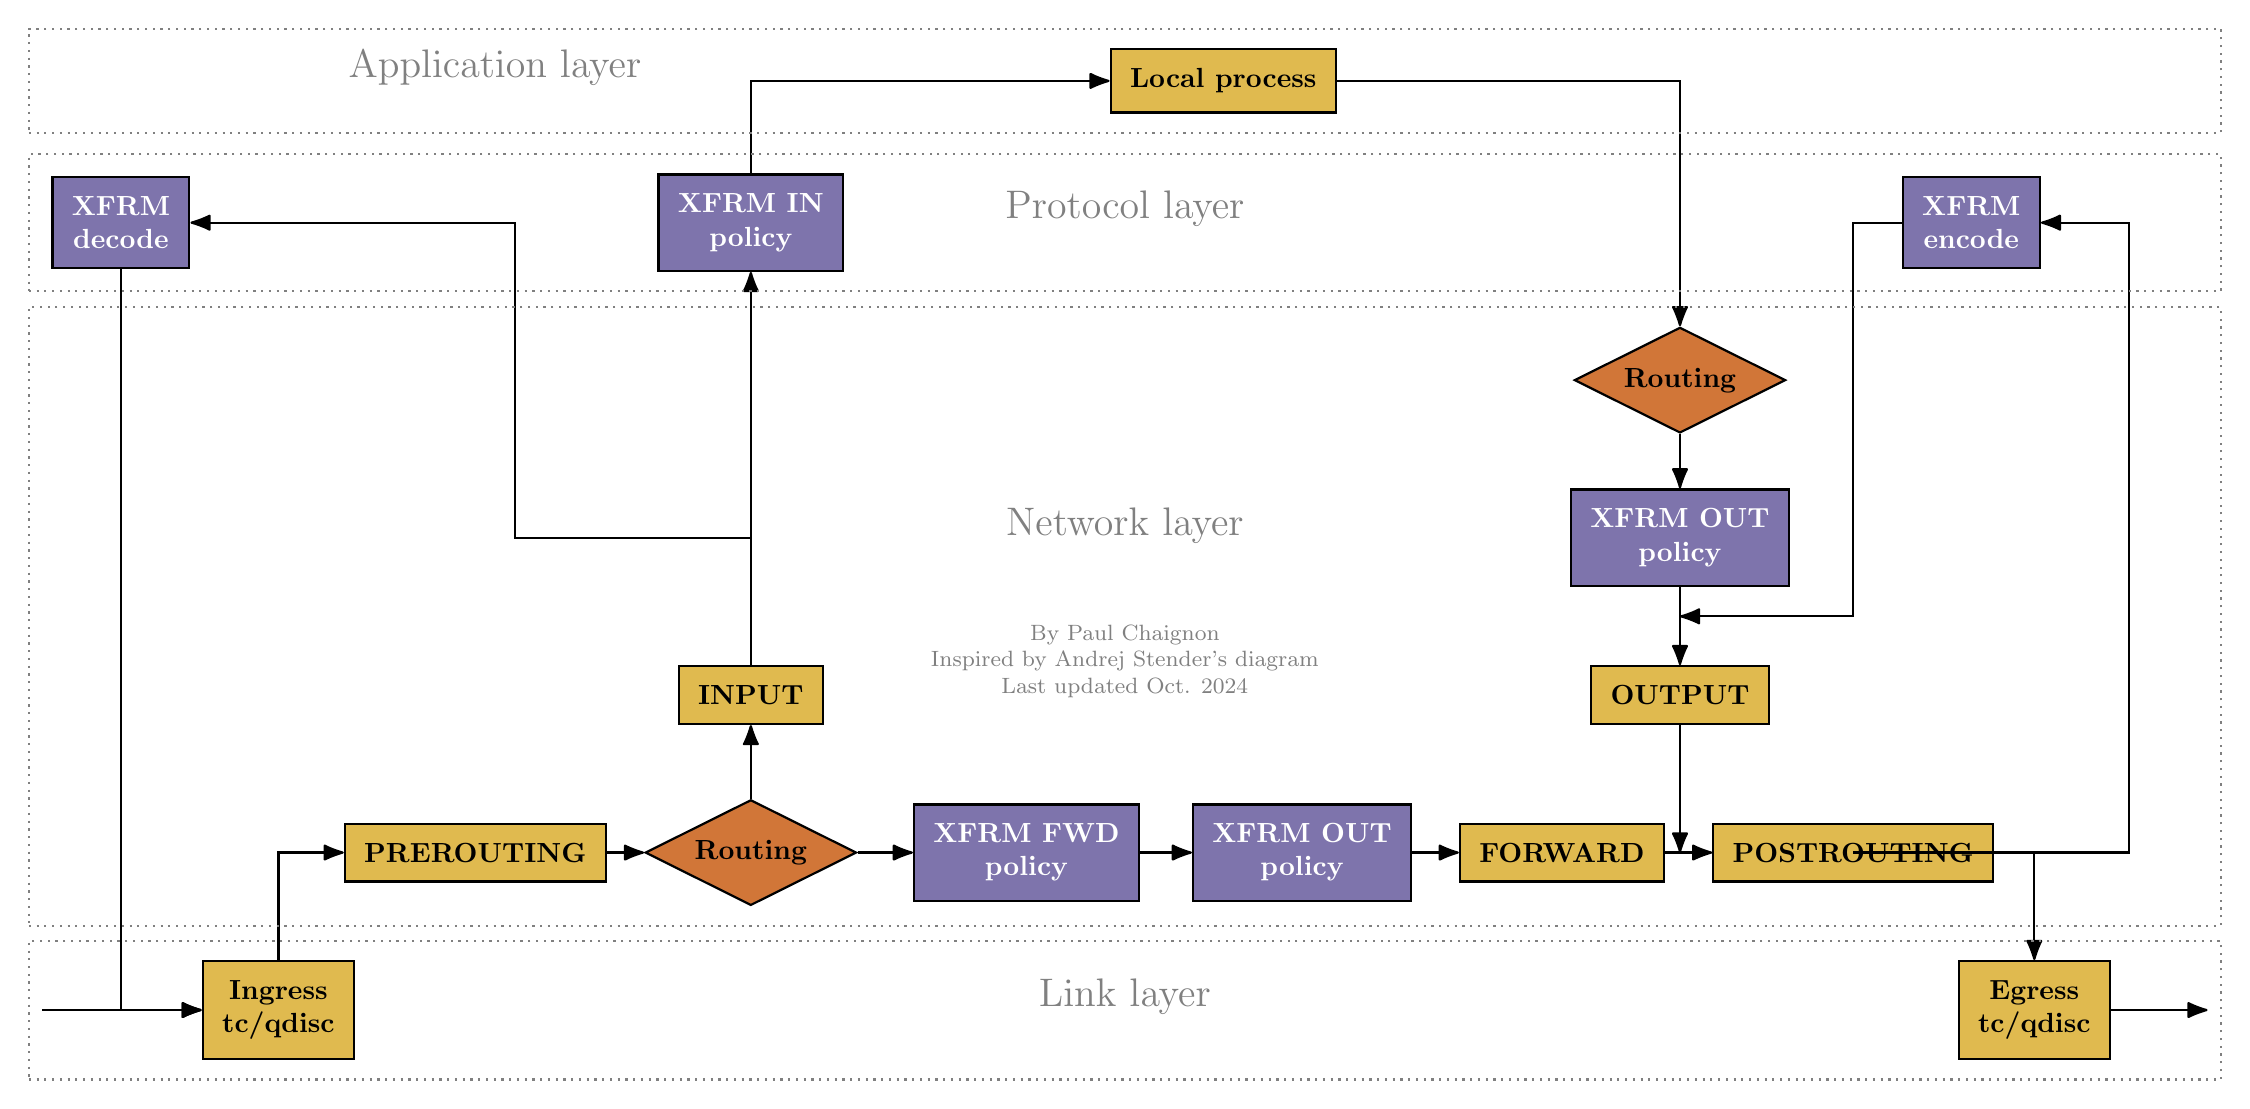
\begin{tikzpicture}
    \tikzset{
        xfrm/.style={rectangle, draw, thick, font=\bfseries, align=center, fill=cpurple, text=white, inner sep=7pt},
        netfilter/.style={rectangle, draw, thick, font=\bfseries, align=center, fill=cyellow, inner sep=7pt},
        routing/.style={diamond, aspect=2, draw, thick, font=\bfseries, align=center, fill=corange, inner sep=3pt},
        layer/.style={rectangle, draw, thick, dotted, font=\Large, gray, inner sep=7pt},
        point/.style={rectangle},
        flow/.style={->, draw, thick, -{Latex[length=3mm, round]}}
    }

    \node[netfilter] (in_tc) at (3, 0) {Ingress\\tc/qdisc};
    \node[netfilter] (prerouting) at (5.5,2) {PREROUTING};
    \node[routing] (in_routing) at (9,2) {Routing};
    \node[xfrm] (fwd_policy) at (12.5,2) {XFRM FWD\\policy};
    \node[xfrm] (out_policy2) at (16,2) {XFRM OUT\\policy};
    \node[netfilter] (forward) at (19.3,2) {FORWARD};
    \node[netfilter] (postrouting) at (23,2) {POSTROUTING};
    \node[netfilter] (out_tc) at (25.3,0) {Egress\\tc/qdisc};
    
    \node[netfilter] (input) at (9,4) {INPUT};
    \node[xfrm] (in_policy) at (9,10) {XFRM IN\\policy};
    
    \node[netfilter] (output) at (20.8,4) {OUTPUT};
    \node[xfrm] (out_policy1) at (20.8,6) {XFRM OUT\\policy};
    \node[routing] (out_routing) at (20.8,8) {Routing};

    \node[xfrm] (encode) at (24.5,10) {XFRM\\encode};

    \node[netfilter] (process) at (15,11.8) {Local process};
    
    \node[xfrm] (decode) at (1,10) {XFRM\\decode};

    \path[flow] (process) -| (out_routing);
    \path[flow] (in_policy) |- (process);
    \path[flow] (out_routing) -- (out_policy1);
    \path[flow] (out_policy1) -- (output);
    \path[flow] (forward) -- (postrouting);
    \path[flow] (input) -- (in_policy);
    \path[flow] (in_routing) -- (input);
    \path[flow] (prerouting) -- (in_routing);
    \path[flow] (fwd_policy) -- (out_policy2);
    \path[flow] (out_policy2) -- (forward);
    \path[flow] (in_routing) -- (fwd_policy);
    \path[flow] (in_tc) |- (prerouting);
    \path[flow] (postrouting) -| (out_tc);
    \path[flow] (decode) |- (in_tc);
    \path[flow] (output) -- (20.8,2);
    \path[flow] (input) |- (6,6) |- (decode);
    \path[flow] (postrouting) |- (26.5,2) |- (encode);
    \path[flow] (encode.west) |- (23,10) |- (20.8,5);
    \path[flow] (0, 0) -- (in_tc);
    \path[flow] (out_tc) -- (27.5,0);

    \node[point] (l2_west) at (0.2,0) {};
    \node[point] (l3_west) at (0.2,6) {};
    \node[point] (l4_west) at (0.2,10) {};
    \node[point] (l7_west) at (0.2,12) {};
    \node[point] (l2_east) at (27.3,0) {};
    \node[point] (l3_east) at (27.3,6) {};
    \node[point] (l4_east) at (27.3,10) {};
    \node[point] (l7_east) at (27.3,12) {};
    \node[layer, fit=(l2_west) (in_tc) (out_tc) (l2_east)] (l2) {Link layer};
    \node[layer, fit=(l3_west) (prerouting) (in_routing) (out_routing) (postrouting) (l3_east)] (l3) {Network layer\\\vspace{1cm}{\footnotesize By Paul Chaignon\\Inspired by Andrej Stender's diagram\\Last updated Oct. 2024\\}};
    \node[layer, fit=(l4_west) (decode) (encode) (in_policy) (l4_east)] (l4) {Protocol layer};
    \node[layer, fit=(l7_west) (process) (l7_east)] (l7) {\hspace{-16cm}Application layer};
\end{tikzpicture}
\end{document}

